\chapter{Introduction}

Introduction

\section{The Standard Model of Particle Physics} \label{sec:standardmodel}

Briefly discuss the history of particle physics (eg Millikan, Rutherford, Planck, Bohr, Dirac\ldots QFT), culminating in the Standard Model.


%  \begin{figure}[h!]
%    \centering
%    \includegraphics[width=\textwidth]{figures/name.pdf}
%    \caption{A caption. \cite{cite_name}}
%    \label{fig:fig_label}
%  \end{figure}  

  Figure \ref{fig:fig_label}

  \subsection{A Brief Description} \label{sec:SMdescription}

  Describe the particles of the Standard Model, and some of their experimental relevance.

  \subsection{Feynman Diagrams} \label{sec:feyndiags}

  Provide a few example Feynman diagrams (eg. ee -> mumu, gg -> top loop -> higgs -> top loop -> gamma gamma) and describe how they represent particle physics processes, and are used to calculate amplitudes. 

  \subsection{Quantum Chromodynamics, Hadronization, and Jets} \label{sec:hadronization}

  Describe why final state quarks and gluons experimentally produce jets. 
  Mention that it is difficult to make precise predictions in QCD (at low energy), leading to requirement for approximate models for jet formation (pythia\ldots).
  In particular, ISR is challenging.

  \subsection{Parton Distribution Functions} \label{sec:PDFs}

  Describe protons as a sea of quarks and gluons with varying momenta, and why we need a PDF to calculate production rates in a hadron collider.

\section{Some Problems with the Standard Model} \label{sec:SMproblems}

Standard Model is extremely successful (electron magnetic moment, Higgs prediction) but not entirely satisfactory.

  \subsection{Effective Field Theory} \label{sec:effective}

  Includes explicit energy cutoff, as part of renormalization.
  Cannot, by contruction, be the final theory.

  \subsection{Gravity} \label{sec:gravity}

  Doesn't include gravity, so Planck scale is maximum possible cutoff (but could be smaller).

  \subsection{The Hierarchy Problem} \label{sec:hierarchy}

  Why is the Higgs mass / weak scale so much smaller than the Planck scale?
  Is the cutoff much smaller?

  \subsection{Astrophysical Evidence of Dark Matter} \label{sec:DMevidence}

  SM has no (cold) dark matter candidate.
  Of course may be well out of reach, but look where we can.
  Good reason to believe that dark matter could be produced at LHC (WIMP miracle).

%  \subsection{The Strong CP Problem} \label{sec:strongCP}

\section{Supersymmetry} \label{sec:SUSY}

SUSY is one particular model that can patches up some of the SM's issues.

  \subsection{Theoretical Appeal} \label{sec:SUSYappeal}

  Solves up hierarchy problem if at the weak scale (so, potentially accessible to LHC) and provides a dark matter candidate.
  (Focus on RPC SUSY, due to proton stability.)

  \subsection{Experimental Signatures} \label{sec:SUSYexp}

  SUSY produces MET, and in strong SUSY decays, potentially lots and lots of jets.
  Since SUSY

  \subsection{Simplified Models} \label{sec:SUSYsms}

  SUSY parameter space is vast, so we consider one potential discovery channel at a time.

  \begin{figure}[h!]
    \centering
    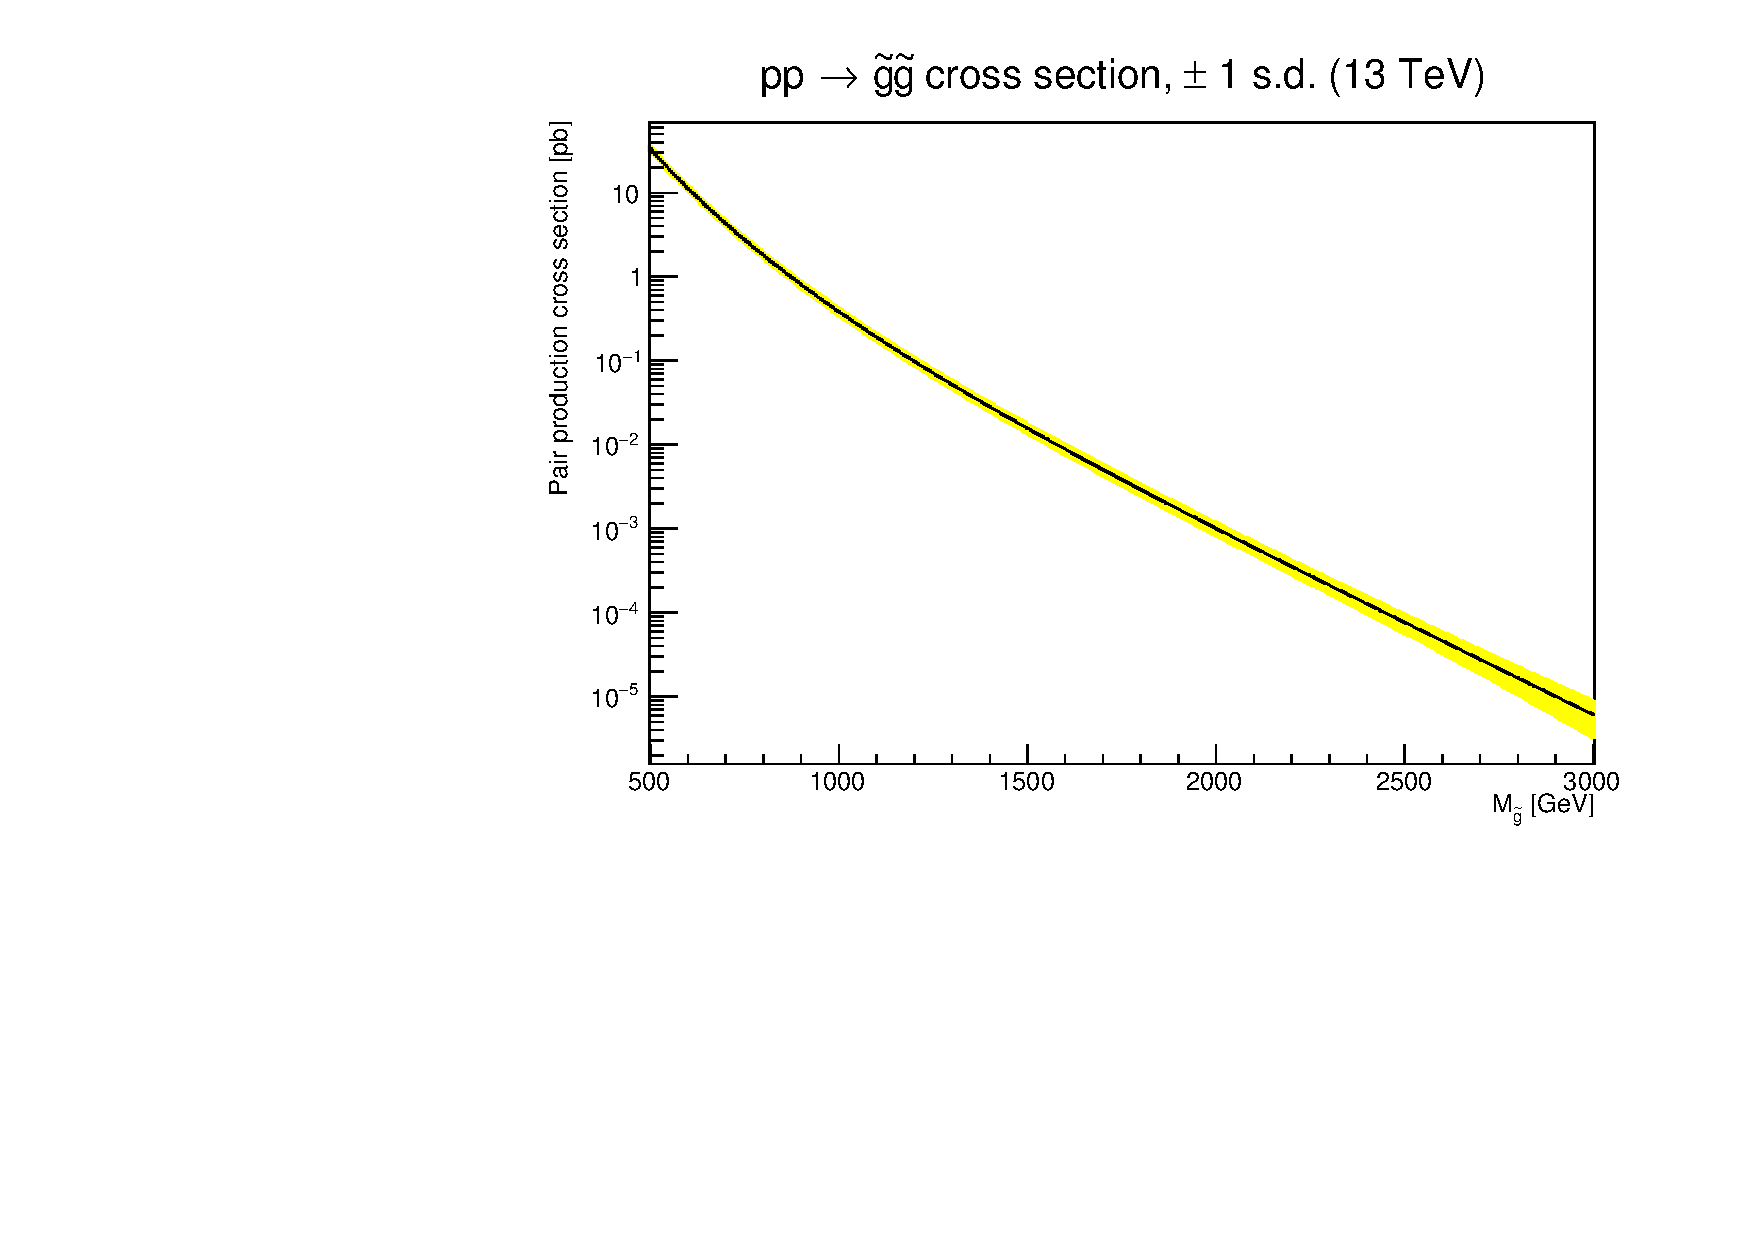
\includegraphics[width=0.85\textwidth]{figures/gluino_xsec.pdf}
    \caption[Theoretical gluino pair production cross section in simplified models.]{In simplified models, it is possible to calculate superpartner production cross sections from theory.
Here, the theoretical gluino pair production cross section in 13 TeV proton-proton collisions is shown in black, with the one standard deviation uncertainty shown as a yellow band.
The cross section drops rapidly with increasing mass.
Based on cross section values used in \cite{MT2_2019}, calculated in \cite{SUSYxsecs}.
Compare Figure 5 (upper) from \cite{SUSYxsecs}, of which this is a simplified reproduction.
}
    \label{fig:SUSYxsec}
  \end{figure}  

\section{Other Models} \label{sec:othermodels}

Introduce leptoquarks and mono-$phi$.

